\section{Produto Vetorial}
 
\subsection{Preliminares}

Antes de definirmos o produto vetorial de dois vetores $\vec{u}$ e $\vec{v}$,
faremos algumas considerações importantes:

\begin{enumerate}[label=\alph*)]
    \item O \textbf{produto vetorial} é um \textbf{vetor}, ao contrário do
      produto escalar $\vec{u} \cdot \vec{v}$, que é um escalar (número real).
    
    \item Para simplicidade de cálculo do produto vetorial, faremos uso de
      \textbf{determinantes}. Um determinante de ordem 2 é definido como:
    \[
      \begin{vmatrix}
        x_1 & y_1 \\
        x_2 & y_2 \\
      \end{vmatrix}
      = x_1y_2 - x_2y_1
    \]
    
    \textbf{Exemplo}:
    \[
      \begin{vmatrix}
        3 & -4 \\
        -2 & 5 \\
      \end{vmatrix}
      = (3)(5) - (-2)(-4) = 15 - 8 = 7
    \]
    
    \item Algumas propriedades dos determinantes serão utilizadas nesta seção:
    \begin{enumerate}[label=\alph{enumi}.\arabic*)]
        \item \textbf{Permutação de linhas}: A troca de duas linhas inverte o
          sinal do determinante.
        
        \textbf{Exemplo}:
        \[
          \begin{vmatrix}
            -4 & 5 \\
            3 & -2 \\
          \end{vmatrix}
          = (-4)(-2) - (3)(5) = 8 - 15 = -7
        \]
        
        \item \textbf{Linhas proporcionais}: Se duas linhas forem constituídas
          de elementos proporcionais, o determinante é zero.
        
        \textbf{Exemplo}:
        \[
          \begin{vmatrix}
            1 & 2 \\
            3 & 6 \\
          \end{vmatrix}
          = (1)(6) - (3)(2) = 6 - 6 = 0
        \]
        
        \item \textbf{Linha nula}: Se uma das linhas for constituída de zeros, o
          determinante é zero.
        
        \textbf{Exemplo}:
        \[
          \begin{vmatrix}
            5 & 7 \\
            0 & 0 \\
          \end{vmatrix}
          = (5)(0) - (0)(7) = 0 - 0 = 0
        \]
    \end{enumerate}
    
    \item Um determinante de ordem 3 pode ser calculado pelo \textbf{Teorema de
      Laplace}:
    \[
      \begin{vmatrix}
        a & b & c \\
        x_1 & y_1 & z_1 \\
        x_2 & y_2 & z_2 
      \end{vmatrix}
      = a\begin{vmatrix}
        y_1 & z_1 \\
        y_2 & z_2 
      \end{vmatrix}
      - b\begin{vmatrix}
        x_1 & z_1 \\
        x_2 & z_2 
      \end{vmatrix}
      + c\begin{vmatrix}
        x_1 & y_1 \\
        x_2 & y_2 
      \end{vmatrix}
    \]
    
    \textbf{Exemplo}:
    \begin{align*}
      \begin{vmatrix}
        3 & 2 & -4 \\
        1 & 3 & 5 \\
        -2 & 1 & 2 
      \end{vmatrix}
      &= 3\begin{vmatrix}
        3 & 5 \\
        1 & 2 
      \end{vmatrix}
      - 2\begin{vmatrix}
        1 & 5 \\
        -2 & 2 
      \end{vmatrix}
      + (-4)\begin{vmatrix}
        1 & 3 \\
        -2 & 1 
      \end{vmatrix} \\
      &= 3(6-5) - 2(2+10) -4(1+6) \\
      &= 3(1) - 2(12) -4(7) \\
      &= 3 - 24 - 28 = -49
    \end{align*}
\end{enumerate}

\begin{center}
\begin{minipage}{0.9\textwidth}
  \textbf{Observação}: O cálculo de determinantes de ordem 3 será fundamental
  para a definição do produto vetorial na próxima seção. O método apresentado
  (Laplace) desenvolve o determinante pela primeira linha, alternando os sinais
  começando por positivo.
\end{minipage}
\end{center}

\subsection{Definição do Produto Vetorial}

Chama-se \textbf{produto vetorial} de dois vetores 
$\vec{u} = x_1\vec{i} + y_1\vec{j} + z_1\vec{k}$ e 
$\vec{v} = x_2\vec{i} + y_2\vec{j} + z_2\vec{k}$, tomados nessa ordem, e se
representa por $\vec{u} \times \vec{v}$, ao vetor:

\begin{equation}
  \vec{u} \times \vec{v} = 
  \begin{vmatrix}
    y_1 & z_1 \\
    y_2 & z_2 
  \end{vmatrix} \vec{i} -
  \begin{vmatrix}
    x_1 & z_1 \\
    x_2 & z_2 
  \end{vmatrix} \vec{j} +
  \begin{vmatrix}
    x_1 & y_1 \\
    x_2 & y_2 
  \end{vmatrix} \vec{k}
  \label{eq:produto_vetorial_def}
\end{equation}

O produto vetorial de $\vec{u}$ por $\vec{v}$ também é indicado por $\vec{u}
\wedge \vec{v}$ e lê-se ``$\vec{u}$ vetorial $\vec{v}$''.

\subsubsection*{Notação Determinantal}

A definição de $\vec{u} \times \vec{v}$ dada em~\eqref{eq:produto_vetorial_def}
pode ser obtida do desenvolvimento segundo o Teorema de Laplace substituindo-se
a primeira linha pelos vetores unitários:

\begin{equation}
  \vec{u} \times \vec{v} = 
  \begin{vmatrix}
    \vec{i} & \vec{j} & \vec{k} \\
    x_1 & y_1 & z_1 \\
    x_2 & y_2 & z_2 
  \end{vmatrix}
  \label{eq:notacao_determinante}
\end{equation}

\begin{center}
\begin{minipage}{0.9\textwidth}
\textbf{Observação}: O símbolo à direita de~\eqref{eq:notacao_determinante} não
  é um determinante verdadeiro, pois a primeira linha contém vetores. No
  entanto, esta notação mnemônica é amplamente utilizada por sua praticidade no
  cálculo do produto vetorial.
\end{minipage}
\end{center}

\subsubsection*{Exemplo de Cálculo}

Calcular $\vec{u} \times \vec{v}$ para $\vec{u} = 5\vec{i} + 4\vec{j} +
3\vec{k}$ e $\vec{v} = \vec{i} + \vec{k}$.

\[
  \vec{u} \times \vec{v} = 
  \begin{vmatrix}
    \vec{i} & \vec{j} & \vec{k} \\
    5 & 4 & 3 \\
    1 & 0 & 1 
  \end{vmatrix}
  = \vec{i} \begin{vmatrix} 4 & 3 \\ 0 & 1 \end{vmatrix} 
  - \vec{j} \begin{vmatrix} 5 & 3 \\ 1 & 1 \end{vmatrix} 
  + \vec{k} \begin{vmatrix} 5 & 4 \\ 1 & 0 \end{vmatrix}
\]

\[
  = \vec{i}(4 \cdot 1 - 3 \cdot 0) - \vec{j}(5 \cdot 1 - 3 \cdot 1) + \vec{k}(5 \cdot 0 - 4 \cdot 1)
\]

\[
  = 4\vec{i} - 2\vec{j} - 4\vec{k}
\]

Portanto:
\[
  \vec{u} \times \vec{v} = 4\vec{i} - 2\vec{j} - 4\vec{k}
\]

\subsection{Dispositivo Prático para o Cálculo de $\vec{u} \times \vec{v}$}

\subsubsection*{Método Mnemônico}

Para calcular o produto vetorial de forma prática:
\begin{enumerate}
  \item Escreva os componentes dos vetores em duas linhas
  \item Repita as duas primeiras colunas à direita
  \item Calcule três determinantes $2 \times 2$ conforme indicado
\end{enumerate}

\begin{center}
\begin{tabular}{ccccc}
  & $\vec{i}$ & $\vec{j}$ & $\vec{k}$ & $\vec{i}$ $\vec{j}$ \\
  $\vec{u}$ & 5 & 4 & 3 & 5 4 \\
  $\vec{v}$ & 1 & 0 & 1 & 1 0 \\
\end{tabular}
\end{center}

Os componentes do produto vetorial são dados por:
\[
  \vec{u} \times \vec{v} = (4\cdot1-3\cdot0)\vec{i} - (5\cdot1-3\cdot1)\vec{j} + (5\cdot0-4\cdot1)\vec{k} = 4\vec{i} - 2\vec{j} - 4\vec{k}
\]

\subsubsection*{Propriedades Fundamentais}
\begin{enumerate}
    \item \textbf{Anti-comutatividade}:
    \begin{equation}
      \vec{v} \times \vec{u} = -(\vec{u} \times \vec{v})
      \label{eq:anti_comutatividade}
    \end{equation}
    O produto vetorial não é comutativo (ao contrário do produto escalar).
    
    \item \textbf{Vetores Paralelos}:
    \begin{equation}
      \vec{u} \times \vec{v} = \vec{0} \iff \vec{u} \parallel \vec{v}
      \label{eq:paralelos}
    \end{equation}
    Casos particulares:
    \begin{itemize}
      \item $\vec{u} \times \vec{u} = \vec{0}$
      \item $\vec{u} \times \vec{0} = \vec{0}$
    \end{itemize}
\end{enumerate}

\subsubsection*{Exemplos de Produto Vetorial Nulo}
\begin{itemize}
  \item $3\vec{u} \times \vec{u} = \vec{0}$
  \item $2\vec{u} \times (-7\vec{u}) = \vec{0}$
  \item $(\vec{u}+\vec{v}) \times (2\vec{u}+3\vec{v}) = \vec{0}$ se $\vec{u} \parallel \vec{v}$
  \item $5\vec{u} \times \vec{0} = \vec{0}$
\end{itemize}

\begin{figure}[h]
  \centering
  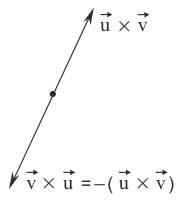
\includegraphics[width=0.4\textwidth]{./fig/fig3.1.png}
  \caption{Ilustração da anti-comutatividade do produto vetorial}
  \label{fig:fig3.1}
\end{figure}

\subsubsection*{Definição Geométrica}

Para vetores não nulos e não paralelos $\vec{u}$ e $\vec{v}$, o vetor $\vec{u}
\times \vec{v}$ é completamente caracterizado por:

\begin{itemize}
  \item \textbf{Direção}: Perpendicular ao plano formado por $\vec{u}$ e $\vec{v}$
  \item \textbf{Sentido}: Regra da mão direita
  \item \textbf{Módulo}: $\|\vec{u} \times \vec{v}\| = \|\vec{u}\|\|\vec{v}\|\sin\theta$
\end{itemize}

\subsection{Características do Vetor $\vec{u} \times \vec{v}$}

Consideremos os vetores $\vec{u} = (x_1, y_1, z_1)$ e $\vec{v} = (x_2, y_2, z_2)$.

\subsubsection*{Direção do Vetor $\vec{u} \times \vec{v}$}
O vetor $\vec{u} \times \vec{v}$ é simultaneamente ortogonal a $\vec{u}$ e $\vec{v}$. Para demonstrar:

\begin{align*}
(\vec{u} \times \vec{v}) \cdot \vec{u} &= 
\begin{vmatrix}
y_1 & z_1 \\
y_2 & z_2 
\end{vmatrix}x_1 - 
\begin{vmatrix}
x_1 & z_1 \\
x_2 & z_2 
\end{vmatrix}y_1 + 
\begin{vmatrix}
x_1 & y_1 \\
x_2 & y_2 
\end{vmatrix}z_1 \\
&= 
\begin{vmatrix}
x_1 & y_1 & z_1 \\
x_1 & y_1 & z_1 \\
x_2 & y_2 & z_2 
\end{vmatrix} = 0 \quad \text{(linhas repetidas)}
\end{align*}

Analogamente, demonstra-se que $(\vec{u} \times \vec{v}) \cdot \vec{v} = 0$.

\begin{figure}[h]
    \centering
    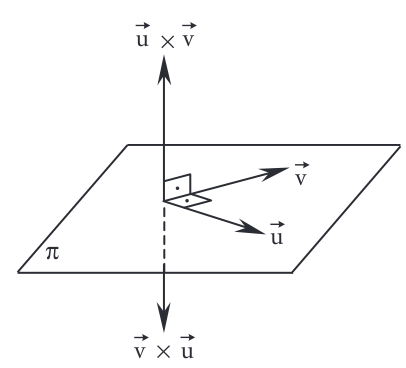
\includegraphics[width=0.4\textwidth]{./fig/fig3.2.png}
    \caption{Ortogonalidade do produto vetorial em relação aos vetores originais}
    \label{fig:fig3.2}
\end{figure}

\subsubsection*{Propriedades Geométricas}
\begin{itemize}
  \item O vetor $\vec{v} \times \vec{u} = -(\vec{u} \times \vec{v})$ tem a mesma direção mas sentido oposto
  \item Ambos são ortogonais ao plano $\pi$ determinado por $\vec{u}$ e $\vec{v}$
  \item A direção segue a \textbf{regra da mão direita}:
    \begin{enumerate}
      \item Posicione a mão direita com os dedos apontando na direção de $\vec{u}$
      \item Dobre os dedos na direção de $\vec{v}$
      \item O polegar estendido aponta na direção de $\vec{u} \times \vec{v}$
    \end{enumerate}
\end{itemize}

\subsubsection*{Interpretação Geométrica}
\begin{center}
\begin{minipage}{0.9\textwidth}
  O produto vetorial $\vec{u} \times \vec{v}$ define um vetor perpendicular ao
  plano que contém $\vec{u}$ e $\vec{v}$, com sentido determinado pela regra da
  mão direita e magnitude igual à área do paralelogramo formado pelos vetores.
\end{minipage}
\end{center}

\subsubsection*{Comprimento do Vetor $\vec{u} \times \vec{v}$}

Se $\theta$ é o ângulo entre os vetores $\vec{u}$ e $\vec{v}$ não nulos, então:

\begin{equation}
  \|\vec{u} \times \vec{v}\| = \|\vec{u}\|\|\vec{v}\|\sin\theta
  \label{eq:norma_produto_vetorial}
\end{equation}

\subsubsection*{Demonstração via Identidade de Lagrange}
Este resultado decorre imediatamente da identidade de Lagrange:

\begin{equation}
  \|\vec{u} \times \vec{v}\|^2 = \|\vec{u}\|^2\|\vec{v}\|^2 - (\vec{u} \cdot \vec{v})^2
  \label{eq:lagrange}
\end{equation}

\subsubsection*{Desenvolvimento Algébrico}
Sabemos que:

\begin{align}
  \|\vec{u} \times \vec{v}\|^2 &= (y_1z_2 - z_1y_2)^2 + (z_1x_2 - x_1z_2)^2 + (x_1y_2 - y_1x_2)^2
  \label{eq:desenvolvimento_norma} \\
  \|\vec{u}\|^2\|\vec{v}\|^2 - (\vec{u} \cdot \vec{v})^2 &= (x_1^2+y_1^2+z_1^2)(x_2^2+y_2^2+z_2^2) - (x_1x_2 + y_1y_2 + z_1z_2)^2
  \label{eq:lagrange_desenvolvido}
\end{align}

A igualdade~\eqref{eq:lagrange} pode ser verificada expandindo ambos os lados
das equações~\eqref{eq:desenvolvimento_norma} e
~\eqref{eq:lagrange_desenvolvido}.

\subsubsection*{Relação com o Ângulo}
Como $\vec{u} \cdot \vec{v} = \|\vec{u}\|\|\vec{v}\|\cos\theta$, podemos
reescrever~\eqref{eq:lagrange} como:

\begin{align*}
  \|\vec{u} \times \vec{v}\|^2 &= \|\vec{u}\|^2\|\vec{v}\|^2 - \|\vec{u}\|^2\|\vec{v}\|^2\cos^2\theta \\
  &= \|\vec{u}\|^2\|\vec{v}\|^2(1 - \cos^2\theta) \\
  &= \|\vec{u}\|^2\|\vec{v}\|^2\sin^2\theta
\end{align*}

Tomando a raiz quadrada e observando que $\sin\theta \geq 0$ para $0^\circ \leq
\theta \leq 180^\circ$, obtemos:

\[
  \|\vec{u} \times \vec{v}\| = \|\vec{u}\|\|\vec{v}\|\sin\theta
\]

\subsubsection*{Interpretação Geométrica}
\begin{itemize}
  \item O módulo do produto vetorial representa a \textbf{área do paralelogramo}
    formado por $\vec{u}$ e $\vec{v}$
  \item Para vetores paralelos ($\theta = 0^\circ$ ou $180^\circ$), $\|\vec{u}
    \times \vec{v}\| = 0$
  \item O valor máximo ocorre quando $\theta = 90^\circ$: $\|\vec{u} \times
    \vec{v}\| = \|\vec{u}\|\|\vec{v}\|$
\end{itemize}

\subsection{Interpretação Geométrica do Módulo do Produto Vetorial}

\subsubsection*{Área do Paralelogramo}
No paralelogramo determinado pelos vetores não nulos $\vec{u}$ e $\vec{v}$:

\begin{itemize}
  \item Base = $\|\vec{u}\|$
  \item Altura = $\|\vec{v}\|\sin\theta$
\end{itemize}

Portanto, a área $A$ do paralelogramo é:

\begin{equation}
  A = \text{base} \times \text{altura} = \|\vec{u}\|\|\vec{v}\|\sin\theta = \|\vec{u} \times \vec{v}\|
  \label{eq:area_paralelogramo}
\end{equation}

\begin{figure}[h]
  \centering
  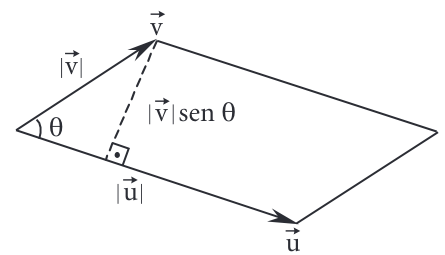
\includegraphics[width=0.4\textwidth]{./fig/fig3.5.png}
  \caption{Paralelogramo formado por $\vec{u}$ e $\vec{v}$ com área $\|\vec{u} \times \vec{v}\|$}
  \label{fig:fig3.5}
\end{figure}

\subsubsection*{Exemplo Ilustrativo}
Considere $\vec{u} = 2\vec{i}$ e $\vec{v} = 3\vec{j}$:

\[
  \vec{u} \times \vec{v} = 
  \begin{vmatrix}
    \vec{i} & \vec{j} & \vec{k} \\
    2 & 0 & 0 \\
    0 & 3 & 0 
  \end{vmatrix}
  = 6\vec{k} \quad \text{e} \quad \|\vec{u} \times \vec{v}\| = 6
\]

A área do paralelogramo é $6$ u.a. (unidades de área), que coincide
numericamente com o comprimento do vetor $6\vec{k}$ (6 u.c.).

\begin{figure}[h]
  \centering
  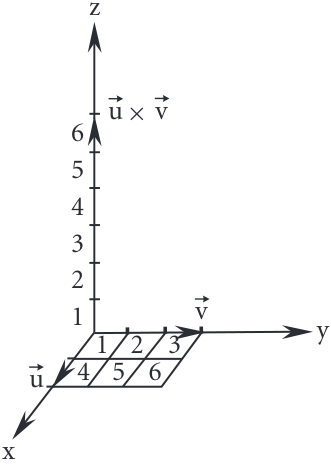
\includegraphics[width=0.3\textwidth]{./fig/fig3.6.png}\label{fig:fig3.6}
\end{figure}

\subsubsection*{Propriedades do Produto Vetorial}
\begin{enumerate}
  \item \textbf{Não associativo}:
    \[
      (\vec{u} \times \vec{v}) \times \vec{w} \neq \vec{u} \times (\vec{v} \times \vec{w})
    \]
    \textbf{Exemplo}:
    \[
      (\vec{i} \times \vec{j}) \times \vec{j} = \vec{k} \times \vec{j} = -\vec{i} \quad \text{enquanto} \quad \vec{i} \times (\vec{j} \times \vec{j}) = \vec{i} \times \vec{0} = \vec{0}
    \]

  \item \textbf{Propriedades algébricas}:
    \begin{itemize}
      \item Distributividade:
        \[
          \vec{u} \times (\vec{v} + \vec{w}) = \vec{u} \times \vec{v} + \vec{u} \times \vec{w}
        \]
        \[
          (\vec{u} + \vec{v}) \times \vec{w} = \vec{u} \times \vec{w} + \vec{v} \times \vec{w}
        \]

      \item Homogeneidade:
        \[
          \alpha(\vec{u} \times \vec{v}) = (\alpha\vec{u}) \times \vec{v} = \vec{u} \times (\alpha\vec{v})
        \]

      \item Identidade do produto misto:
        \[
          \vec{u} \cdot (\vec{v} \times \vec{w}) = (\vec{u} \times \vec{v}) \cdot \vec{w}
        \]
    \end{itemize}
\end{enumerate}

\begin{center}
\begin{minipage}{0.9\textwidth}
  \textbf{Desafio}: Demonstre as propriedades acima utilizando a definição do
  produto vetorial e propriedades de determinantes.
\end{minipage}
\end{center}

\subsubsection*{Demonstrações das Propriedades do Produto Vetorial}

Sejam os vetores $\vec{u} = (u_1, u_2, u_3)$, $\vec{v} = (v_1, v_2, v_3)$ e $\vec{w} = (w_1, w_2, w_3)$.

\begin{enumerate}
  \item \textbf{Não associatividade}:
  
  O produto vetorial não é associativo, ou seja:
  \[
    (\vec{u} \times \vec{v}) \times \vec{w} \neq \vec{u} \times (\vec{v} \times \vec{w})
  \]

  \textbf{Exemplo:} Seja $\vec{u} = \vec{i}$, $\vec{v} = \vec{j}$ e $\vec{w} = \vec{j}$. Então:
  \[
    (\vec{i} \times \vec{j}) \times \vec{j} = \vec{k} \times \vec{j} = -\vec{i}
  \quad \text{enquanto} \quad
    \vec{i} \times (\vec{j} \times \vec{j}) = \vec{i} \times \vec{0} = \vec{0}
  \]

  Como $-\vec{i} \neq \vec{0}$, concluímos que o produto vetorial não é
    associativo.

  \item \textbf{Propriedades algébricas:}
  
  \begin{itemize}
    \item \textbf{Distributividade:}
    \[
      \vec{u} \times (\vec{v} + \vec{w}) = \vec{u} \times \vec{v} + \vec{u} \times \vec{w}
    \]
    \[
      (\vec{u} + \vec{v}) \times \vec{w} = \vec{u} \times \vec{w} + \vec{v} \times \vec{w}
    \]
    
    \textbf{Demonstração:} A definição do produto vetorial via determinante nos dá:
    \[
    \vec{u} \times \vec{v} =
    \begin{vmatrix}
    \vec{i} & \vec{j} & \vec{k} \\
    u_1 & u_2 & u_3 \\
    v_1 & v_2 & v_3
    \end{vmatrix}
    \]
    
    Substituindo $\vec{v} + \vec{w}$ na segunda linha do determinante, e usando
      a linearidade da operação, obtemos a distributividade.

    \item \textbf{Homogeneidade:}
    \[
      \alpha(\vec{u} \times \vec{v}) = (\alpha \vec{u}) \times \vec{v} = \vec{u} \times (\alpha \vec{v})
    \]

    \textbf{Demonstração:} Como o produto vetorial é bilinear, o escalar
      $\alpha$ pode ser colocado em evidência:
    \[
    \alpha(u_2v_3 - u_3v_2) = (\alpha u_2)v_3 - (\alpha u_3)v_2
    \]
    Portanto, a multiplicação escalar pode ser aplicada a qualquer um dos
    vetores, mas nunca em dois ao mesmo tempo.

    \item \textbf{Produto misto (identidade):}
    \[
      \vec{u} \cdot (\vec{v} \times \vec{w}) = (\vec{u} \times \vec{v}) \cdot \vec{w}
    \]

    \textbf{Demonstração:} Ambos os lados resultam no determinante:
    \[
    \begin{vmatrix}
    u_1 & u_2 & u_3 \\
    v_1 & v_2 & v_3 \\
    w_1 & w_2 & w_3
    \end{vmatrix}
    \]
    que representa o volume assinado do paralelepípedo formado pelos vetores
    $\vec{u}$, $\vec{v}$ e $\vec{w}$.
  \end{itemize}
\end{enumerate}

\newpage
\subsection{Uma Aplicação na Física}

O produto vetorial é uma importante ferramenta matemática utilizada na Física.
Entre suas aplicações, destaca-se o cálculo do \textbf{torque}.

\subsubsection*{Definição de Torque}
O torque ($\vec{\tau}$) é uma grandeza vetorial relacionada à capacidade de uma
força causar rotação em um corpo:

\begin{equation}
  \vec{\tau} = \vec{r} \times \vec{F}
  \label{eq:torque}
\end{equation}

onde:
\begin{itemize}
  \item $\vec{r}$ é o vetor posição (do eixo de rotação ao ponto de aplicação da
    força)
  \item $\vec{F}$ é a força aplicada
  \item $\|\vec{r}\|$ é a distância do eixo de rotação
\end{itemize}

\subsubsection*{Módulo do Torque}
Pela equação \eqref{eq:torque} e usando a fórmula do módulo do produto vetorial:

\begin{equation}
  \|\vec{\tau}\| = \|\vec{r}\|\|\vec{F}\|\sin\theta
  \label{eq:modulo_torque}
\end{equation}

onde $\theta$ é o ângulo entre $\vec{r}$ e $\vec{F}$.

\begin{center}
\begin{minipage}{0.9\textwidth}
  \textbf{Observação}: Embora torque e trabalho tenham a mesma unidade (N·m),
  são grandezas físicas distintas - torque é vetorial enquanto trabalho é
  escalar.
\end{minipage}
\end{center}
